\documentclass{beamer}

%\usetheme{PaloAlto}
\usetheme{AnnArbor}

\graphicspath{{./Bilder/},{../Session_1/Bilder}}
\usepackage{blindtext}
\usepackage{booktabs}
\usepackage{lpic}

\usepackage{etoolbox}

%https://tex.stackexchange.com/questions/170268/separation-space-between-tableofcontents-items-in-beamer
\makeatletter
\patchcmd{\beamer@sectionintoc}
  {\vfill}
  {\vskip\itemsep}
  {}
  {}
\makeatother  

\title{Quanten und Photonen}
\subtitle{Eine Einführung}

\author{Uwe Ziegenhagen}
\institute{DLR}

\begin{document}

\begin{frame}
\maketitle
\end{frame}

\begin{frame}
\frametitle{Inhalt}

\tableofcontents


\end{frame}

\section{Einführung}

\begin{frame}[allowframebreaks]
\frametitle{Hallo DLR}
\framesubtitle{Beamer ist toll}

\blindtext[2]

\end{frame}

\begin{frame}
\frametitle{Aufzählungen}

\begin{itemize}
\item Hallo
\item ich 
\item bin 
\item eine 
\item Aufzählungsliste
\item Hallo Welt
\end{itemize}
\end{frame}

\begin{frame}
\frametitle{Aufzählungen}

\begin{enumerate}[I]
\item Hallo
\item ich 
\item bin 
\item eine 
\item Aufzählungsliste
\item Hallo Welt
\end{enumerate}
\end{frame}

\section{Bilder}

\begin{frame}
\frametitle{Bilder}

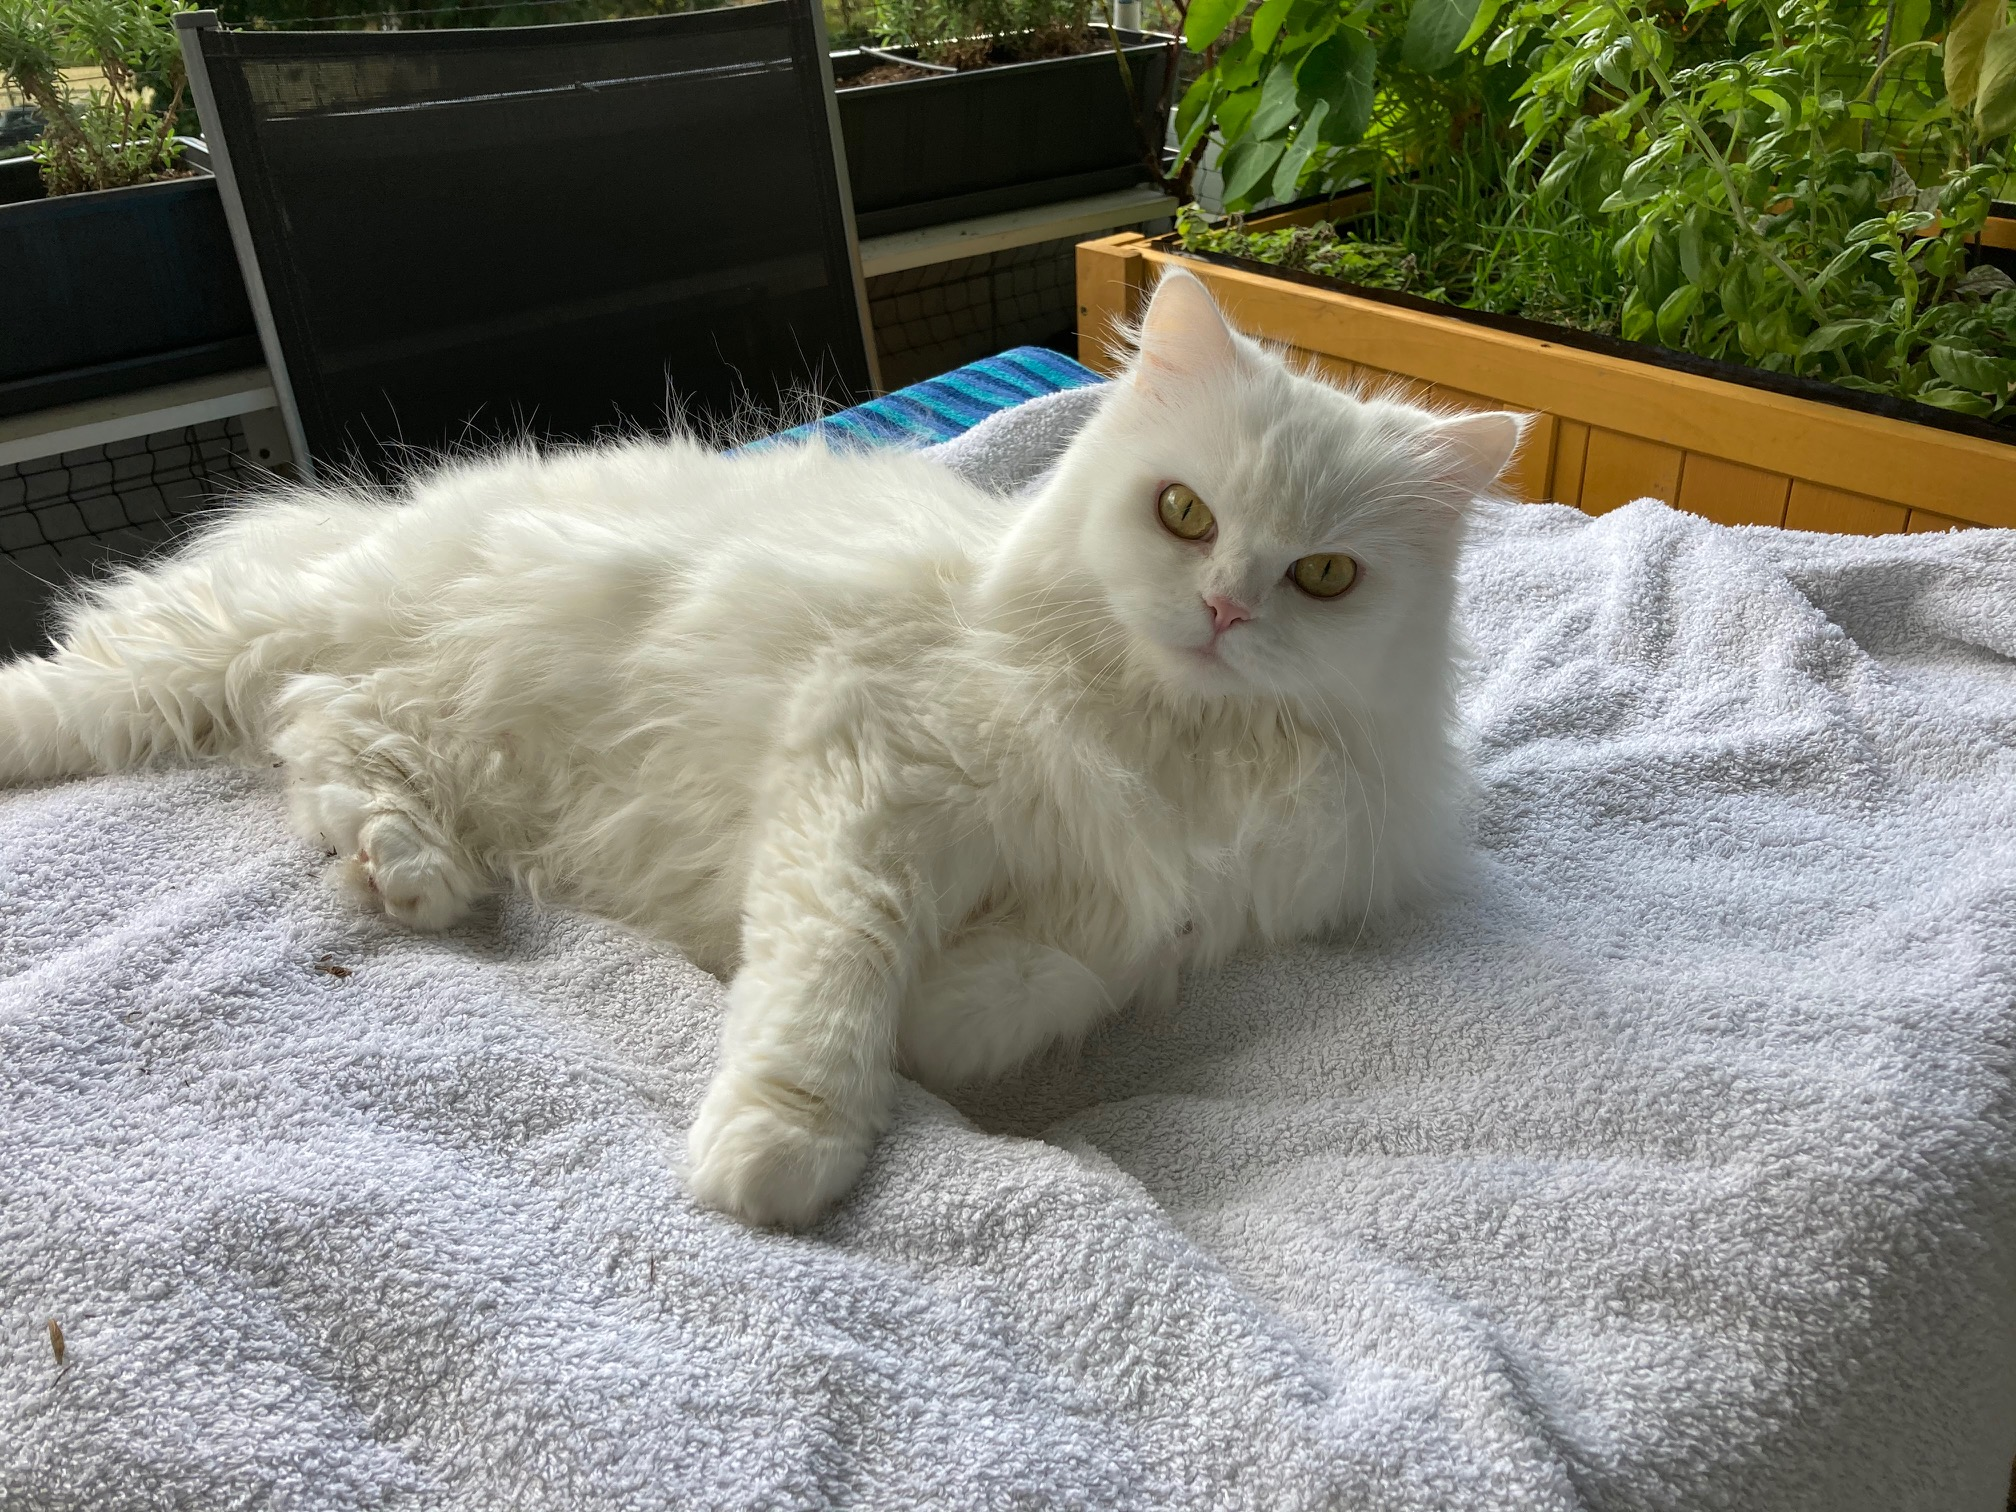
\includegraphics[width=\textwidth]{Katze1}


\end{frame}

\begin{frame}
\frametitle{Bilder}

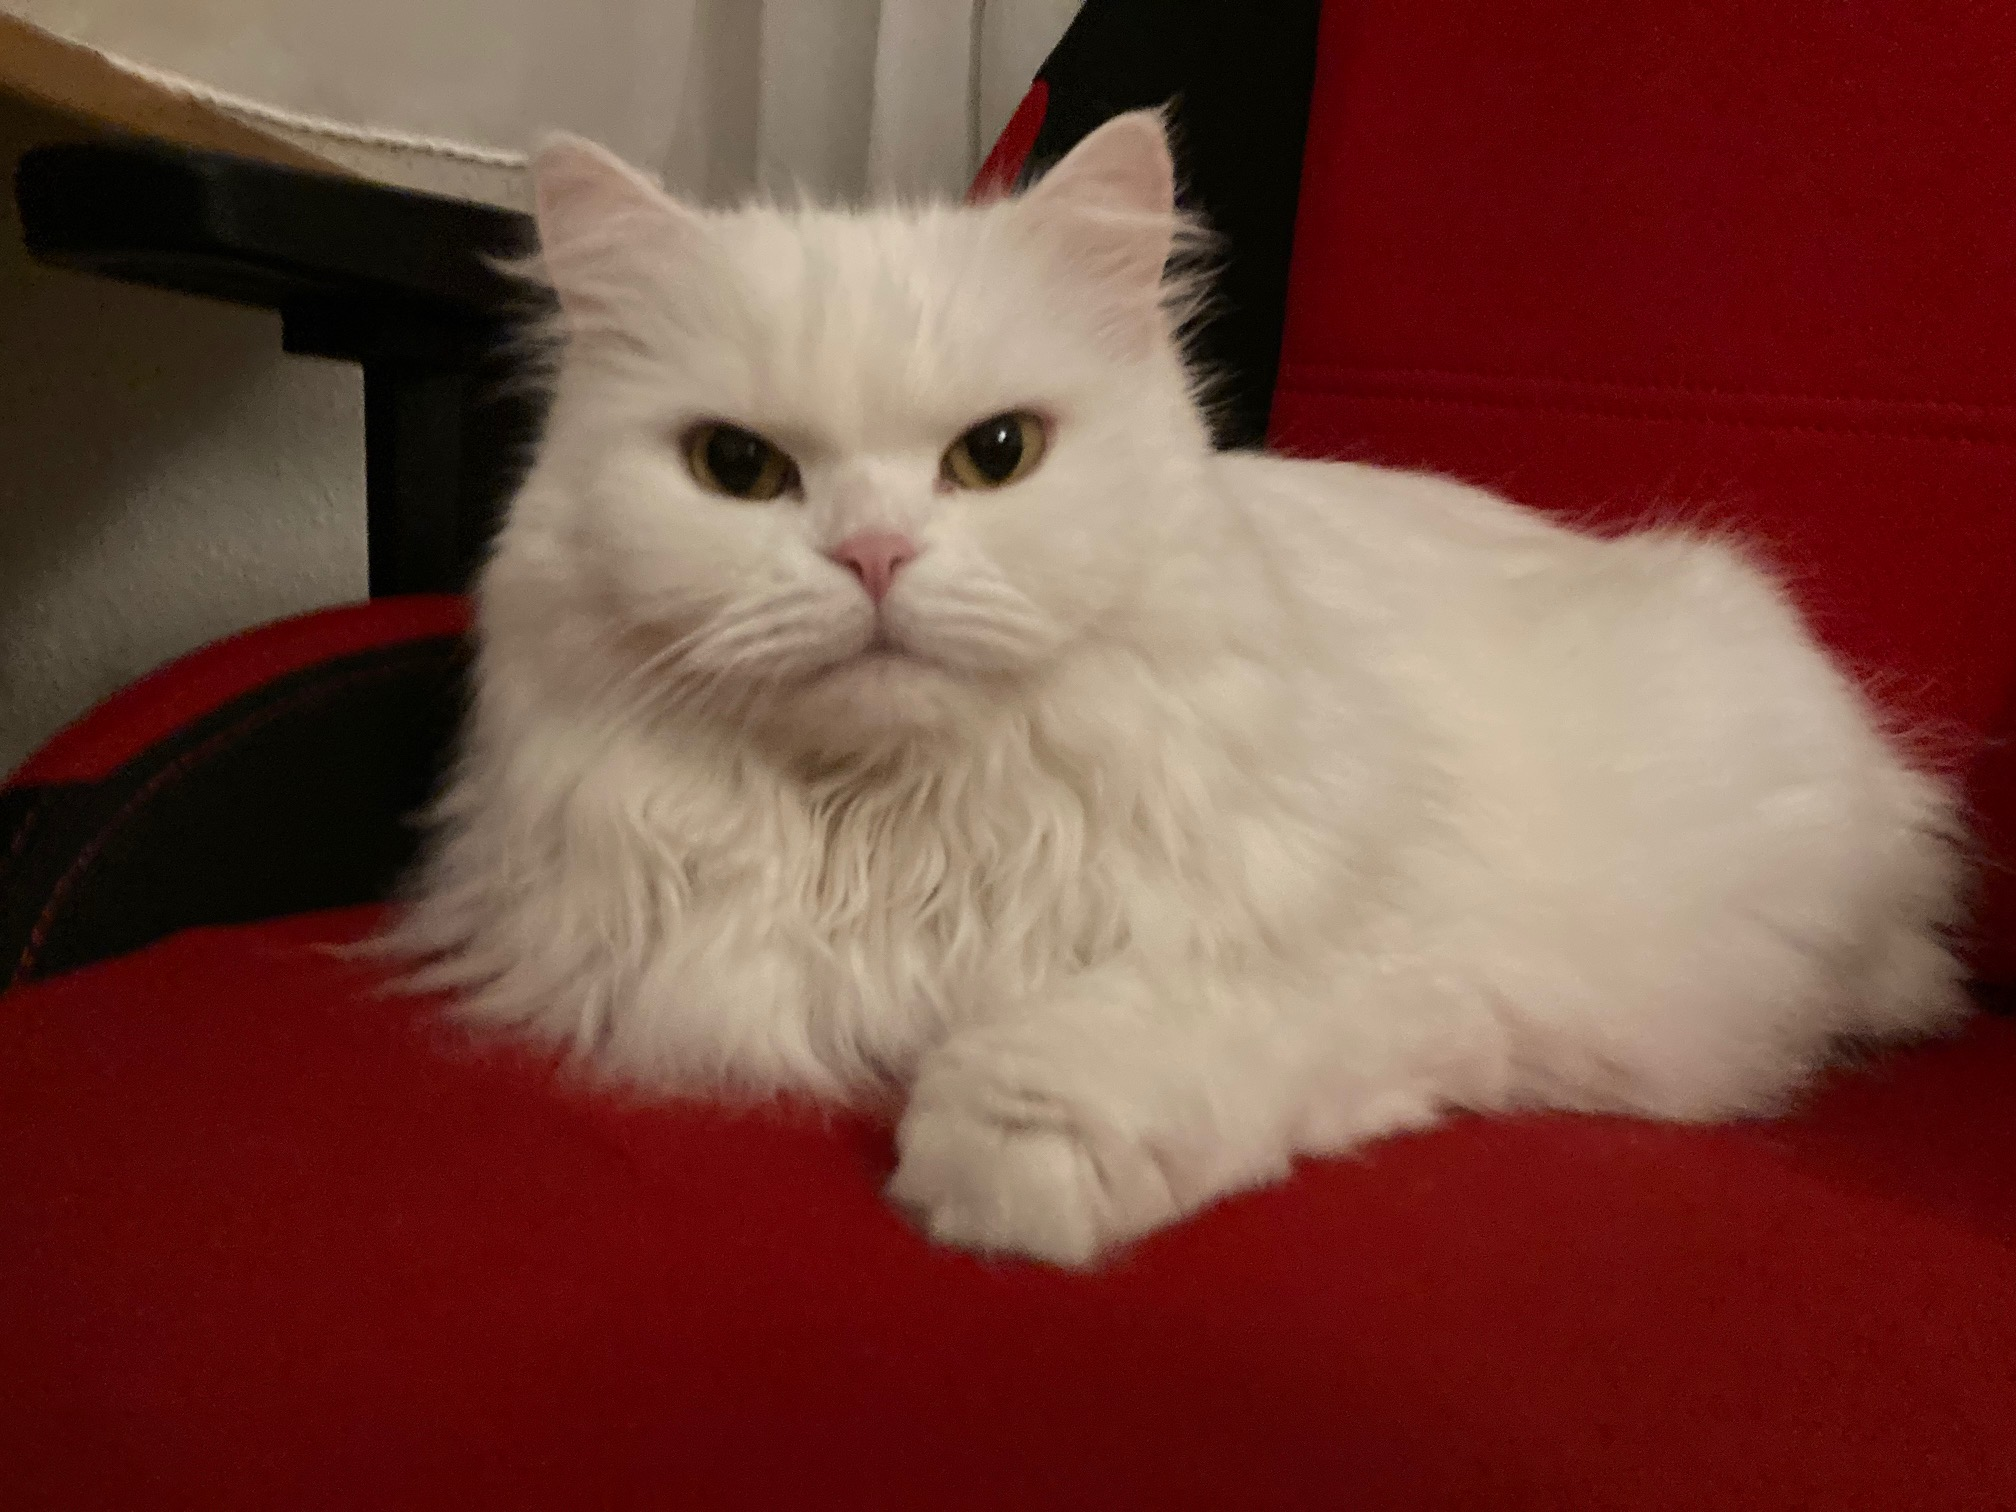
\includegraphics[width=\textwidth]{Katze}

\end{frame}

\begin{frame}
\frametitle{Bilder}

\begin{columns}
\begin{column}{0.5\textwidth}
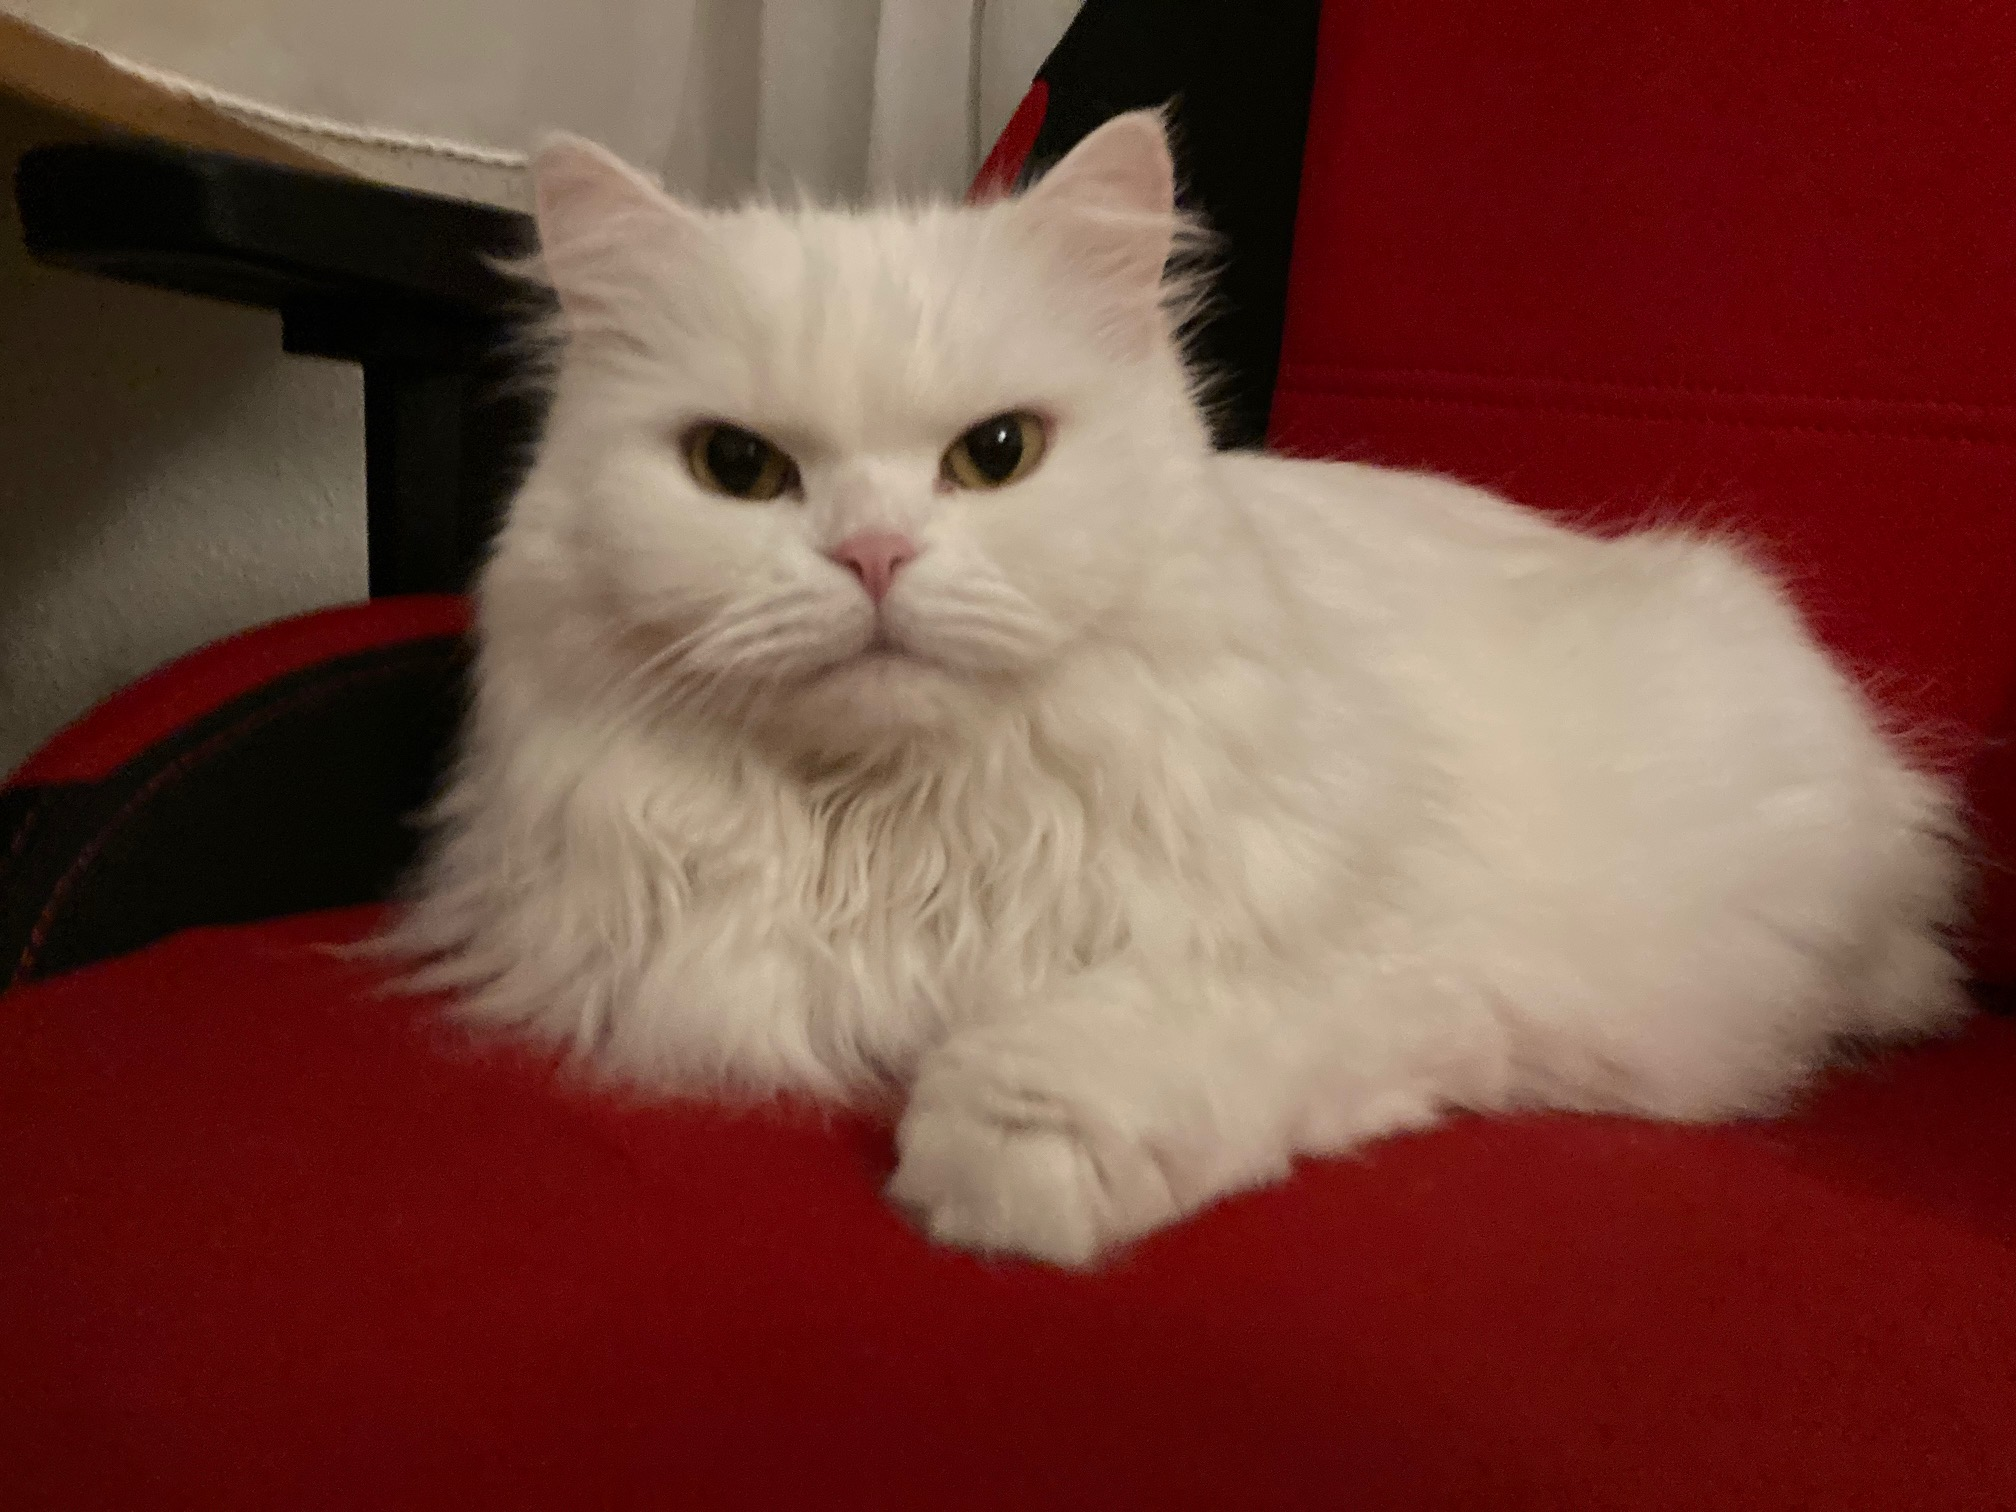
\includegraphics[width=\textwidth]{Katze}
\end{column}
\begin{column}{0.5\textwidth}
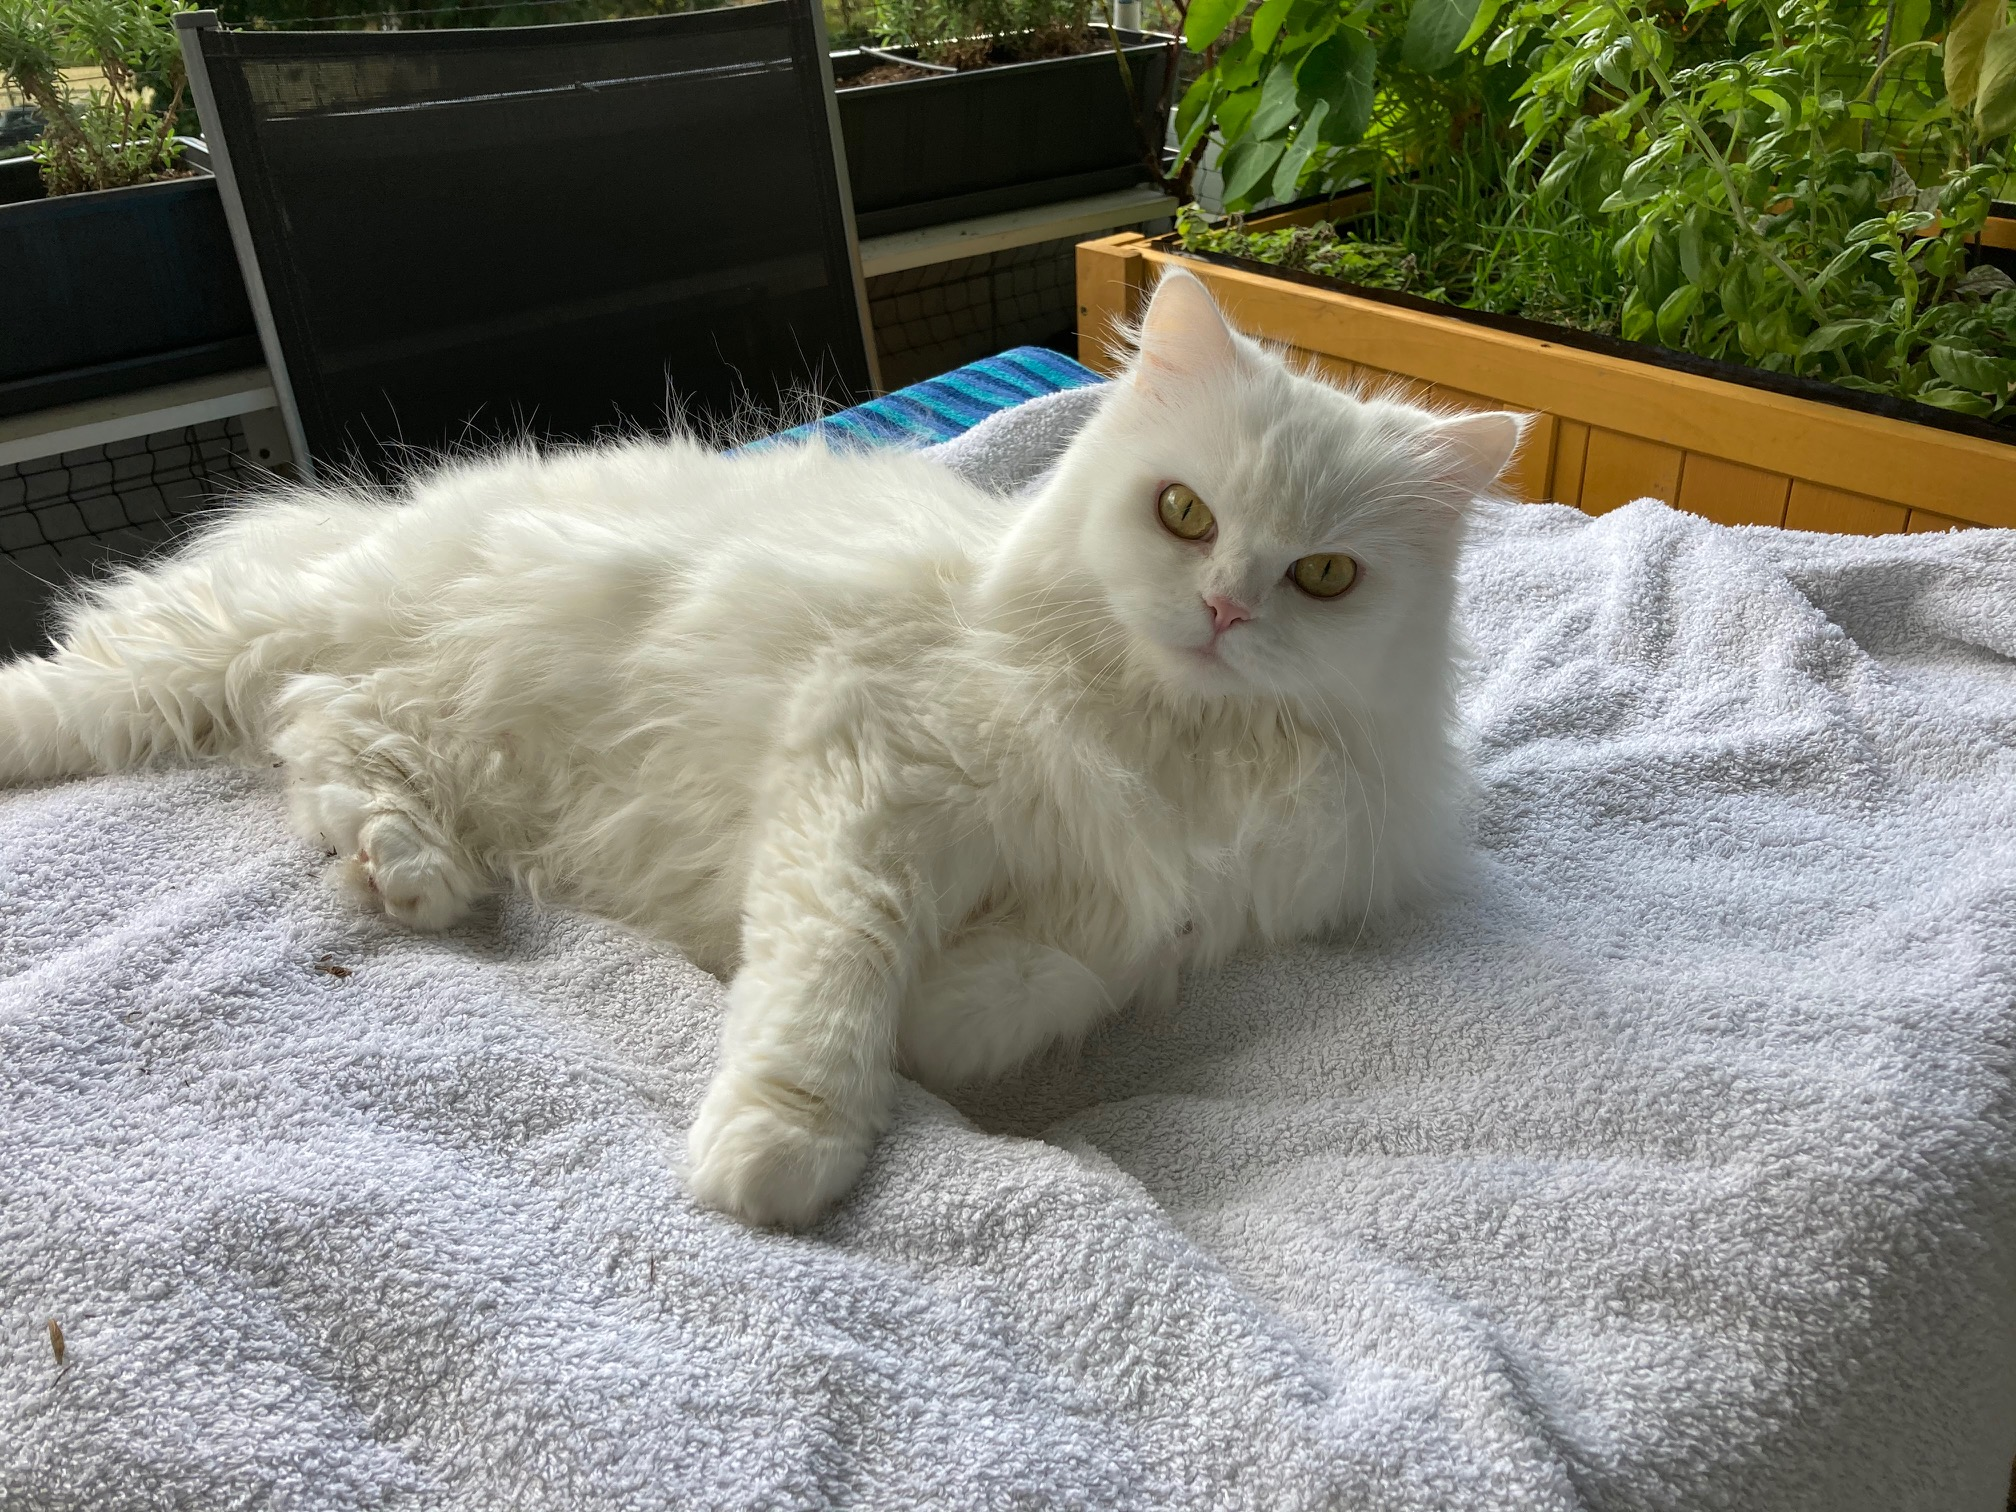
\includegraphics[width=\textwidth]{Katze1}
\end{column}
\end{columns}

\end{frame}

\begin{frame}
\frametitle{Bilder}

\begin{columns}
\begin{column}{0.33\textwidth}
\begin{itemize}
	\item 
	\item 
	\item 
	\item 
	\item 
	\item 
	\end{itemize}
\end{column}
\begin{column}{0.33\textwidth}
\begin{itemize}
	\item 
	\item 
	\item 
	\item 
	\item 
	\item 
	\end{itemize}
\end{column}
\begin{column}{0.33\textwidth}
\begin{itemize}
	\item 
	\item 
	\item 
	\item 
	\item 
	\item 
	\end{itemize}
\end{column}
\end{columns}
\end{frame}

\subsection{Fazit}

\begin{frame}
\frametitle{Mathe}

\(a+b=c\)

\[-\frac{p}{2} \pm \sqrt{ \left(\frac{p}{2}\right)^2 -q  }\]

\scalebox{5}{\rotatebox{45}{Hallo DLR}}

\end{frame}

\section{Booktabs}

\begin{frame}
\frametitle{Booktabs}

\begin{tabular}{|l|c|r|p{4cm}|} \hline
Spalte 1 & Spalte 2 & Spalte 3 & Spalte 4 \\ \hline
aaa & bb & ccc & dddd \\ \hline
wefsdfsfs & sdfsdfsdfsd & sdfsdfsdf & fsdfsdfsdfs\\ \hline
wefsdfsfs & sdfsdfsdfsd & sdfsdfsdf & fsdfsdfsdfs\\ \hline
wefsdfsfs & sdfsdfsdfsd & sdfsdfsdf & fsdfsdfsdfs\\ \hline
wefsdfsfs & sdfsdfsdfsd & sdfsdfsdf & fsdfsdfsdfs\\ \hline
\end{tabular}

\end{frame}

\begin{frame}
\frametitle{Booktabs}

\begin{tabular}{lcrp{4cm}} \toprule[1.5pt]
\textbf{Spalte 1} & \textbf{Spalte 2} & \textbf{Spalte 3} & \textbf{Spalte 4} \\ \midrule
aaa & bb & ccc & dddd \\ \cmidrule[1pt](lr){1-4}
wefsdfsfs & sdfsdfsdfsd & sdfsdfsdf & fsdfsdfsdfs\\ 
wefsdfsfs & sdfsddfsd & sdfsdfsdf & fsdfsdfsdfs\\ \addlinespace[0.5em]
wefsdfsfs & sdfsdfsdfsd & sddfsdf & fsdfss\\ 
wefsdfsfs & sdfsdfsdfsd & sdfsdfsdf & fsdfsdfsdfs\\ \bottomrule[1.5pt]
\end{tabular}

\end{frame}

\begin{frame}
\frametitle{Bilder}
\begin{center}
\begin{lpic}[]{Katze(0.15)} % grid, coords(20)
\lbl[t]{200,500;\textcolor{yellow}{\small \textbf{Ohr 1}}}
\lbl[t]{115,150;\textcolor{green}{\small \textbf{Atmega 16U2}}}
\lbl[t]{54,38;\textcolor{green}{\textbf{7--12V}}}
\lbl[t]{195,66;\textcolor{green}{\textbf{ATMega 328}}}
\lbl[t]{200,20;\textcolor{green}{\textbf{IO-Ports}}}
\lbl[t]{200,195;\textcolor{green}{\textbf{IO-Ports}}}
\end{lpic}
\end{center}

\end{frame}

\begin{frame}
\frametitle{Aufdecken von }

\begin{itemize}
\item<1-2> ABD
\item<-3> fdsgfd
\item<1-> dfgfdgfd
\item<2,4> gdfgfdg
\item dfgfdgfd
\item dfgdfgdf
\end{itemize}
\end{frame}

\begin{frame}
\frametitle{}

\cite{Knuth}

\begin{theorem}
There is no largest prime number.
\end{theorem}

\begin{proof}
There is no largest prime number.
\end{proof}

\begin{alert}{Wichtig}
There is no largest prime number.
\end{alert}

\begin{alertblock}{Wrong Theorem}
$1=2$.
\end{alertblock}

\end{frame}

\begin{frame}
\frametitle{}

\begin{thebibliography}
\setbeamertemplate{bibliography item}[book]
\bibitem{Knuth} Donald Knuth
\end{thebibliography}


\end{frame}



\end{document}


\begin{frame}
\onslide<1>
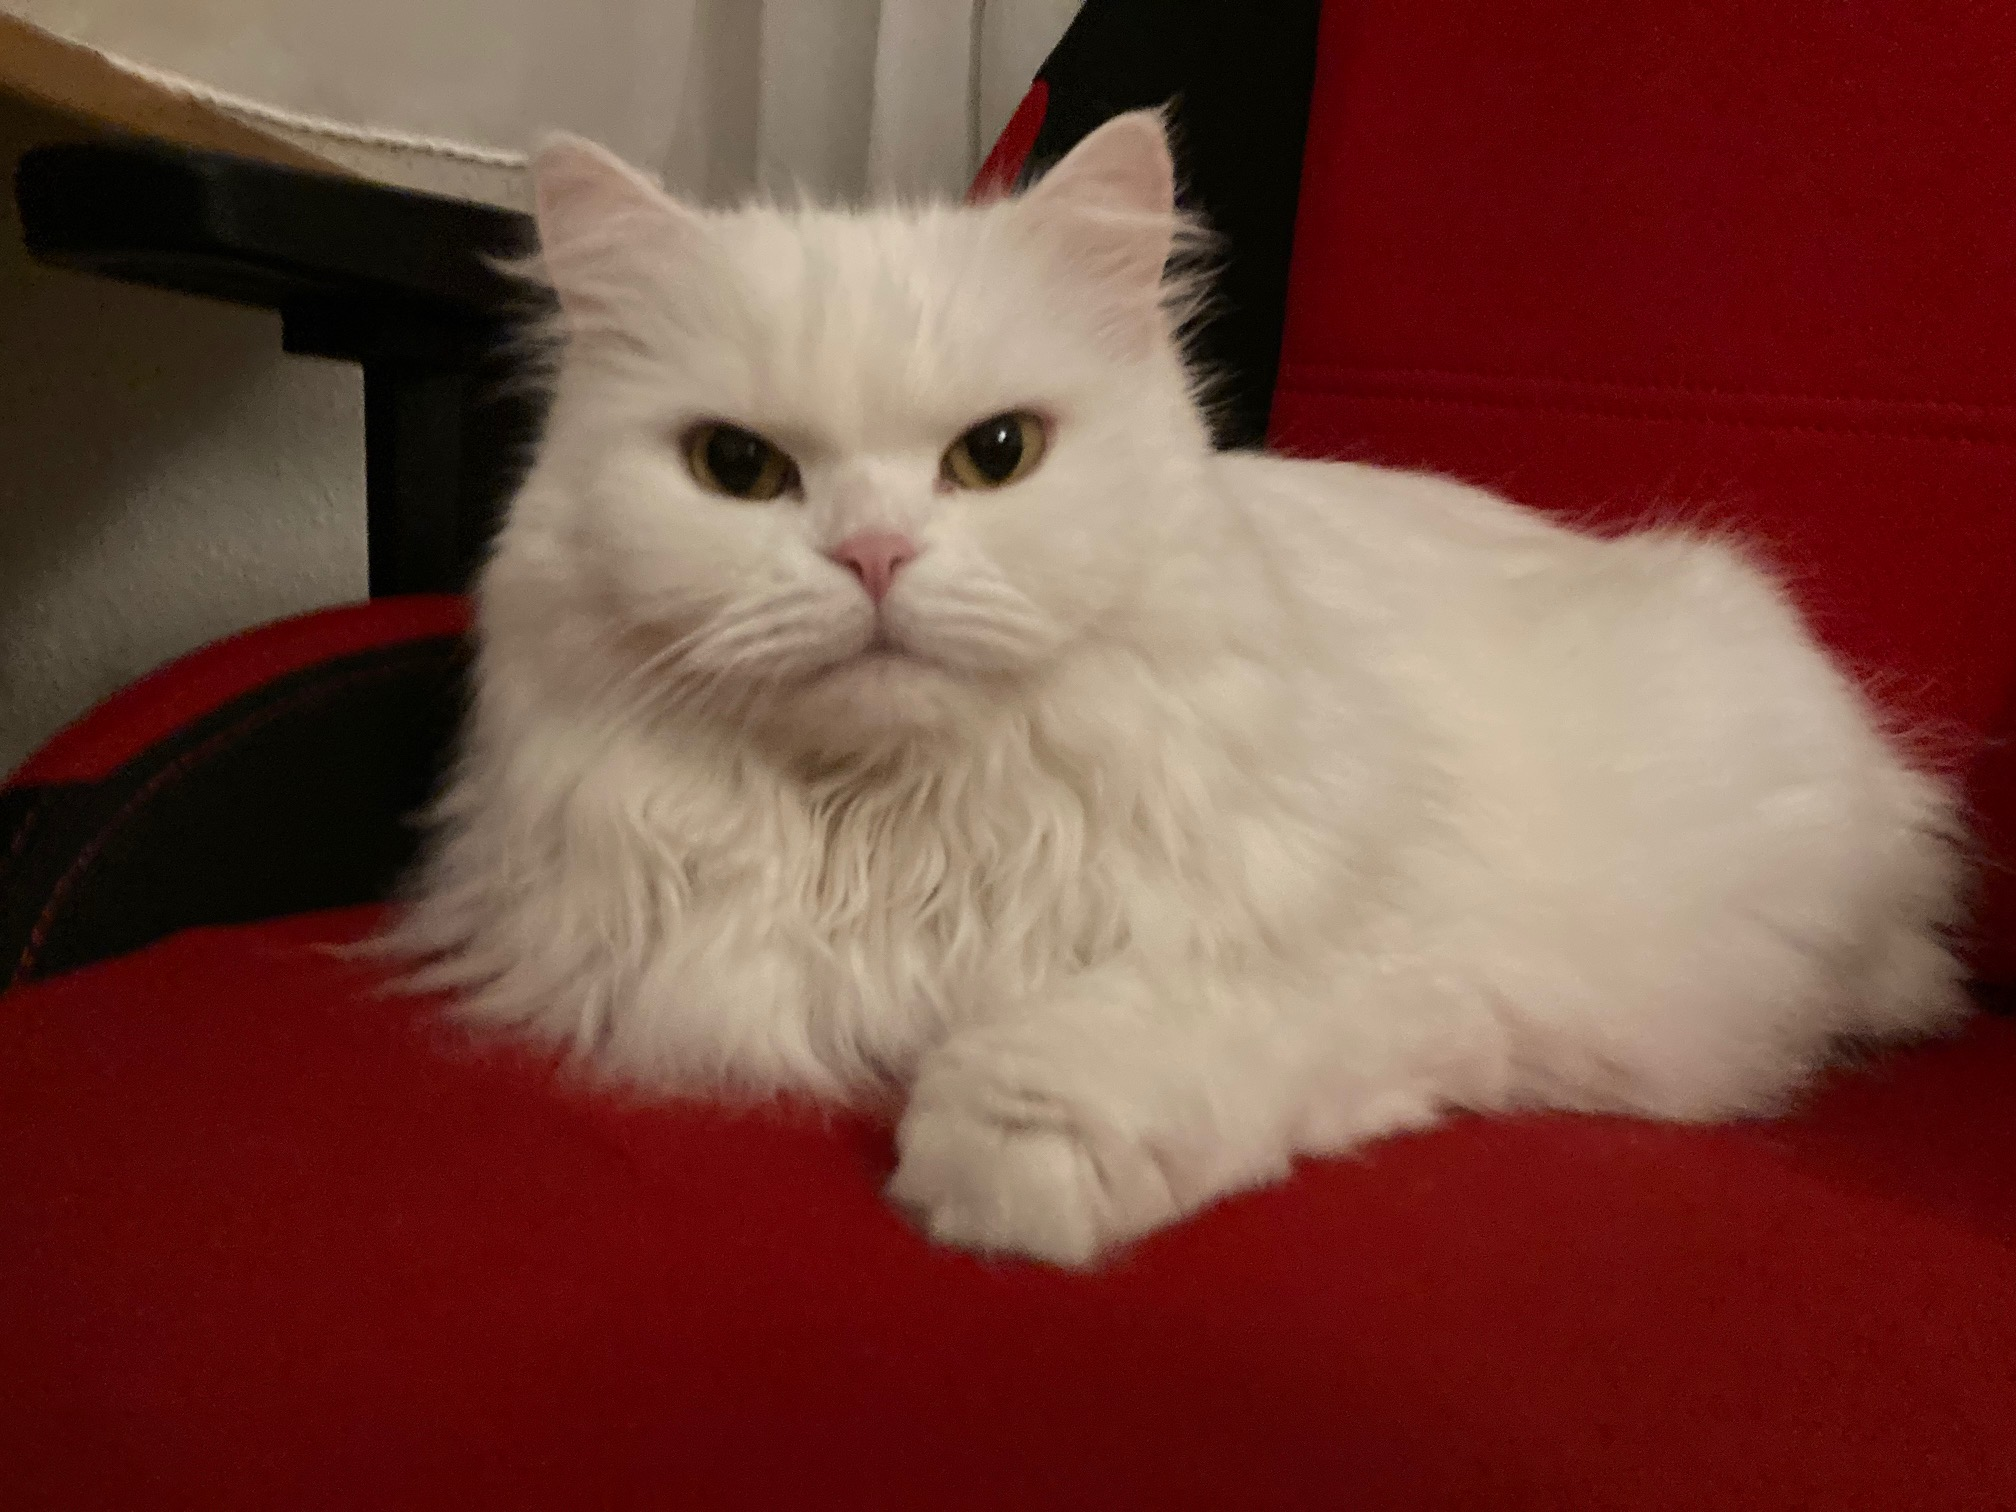
\includegraphics[width=\textwidth]{Katze}
\onslide<2>
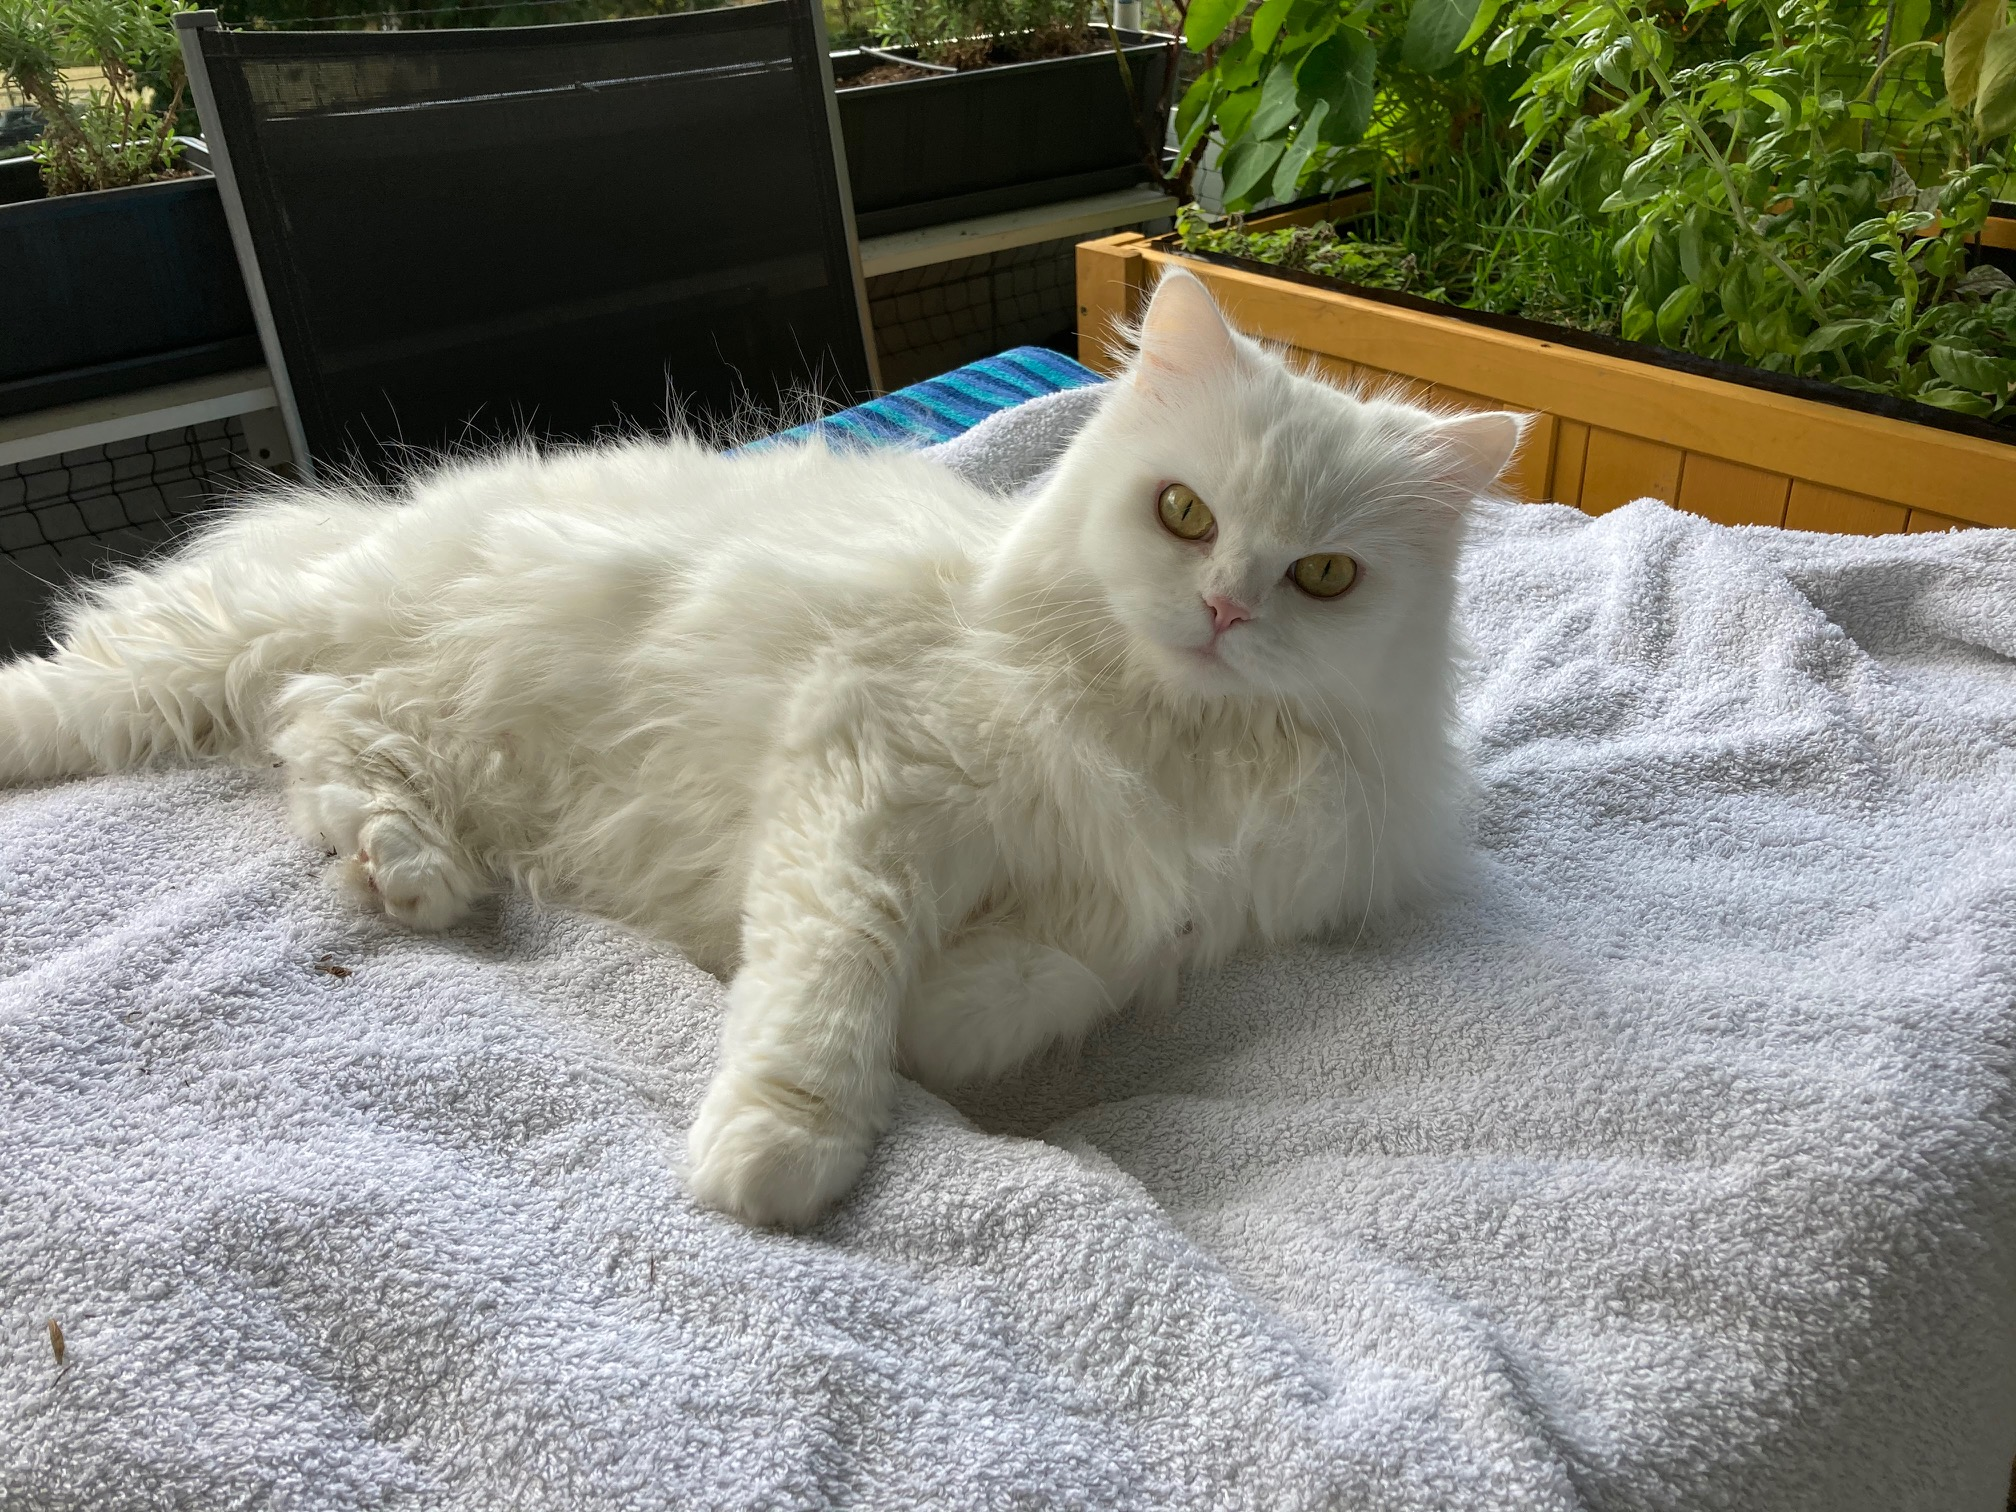
\includegraphics[width=\textwidth]{Katze1}
\end{frame}
